\documentclass[sigconf,nonacm]{acmart}

% ---------------------------------------------------------------------------
% Numbers policy for this paper: every number in the text and in every table
% comes from results/*.csv in the accompanying artefact. Tables are generated
% by src/make_paper_tex.py, and tests/check_paper.py fails when a number in the
% .tex stops matching the CSV. Do not type a number by hand here.
% ---------------------------------------------------------------------------

\usepackage{booktabs}
\usepackage{graphicx}
\usepackage{amsmath}
\usepackage{xcolor}
\usepackage{tikz}
\usetikzlibrary{arrows.meta,positioning,shapes.geometric}

\newcommand{\todo}[1]{\textcolor{red}{[TODO: #1]}}

% Cross-references are spelled out as "Section~N" rather than "\S N", so the
% word itself must not break across a line as "Sec-" + "tion".
\hyphenation{Section}

% A figure drawn in TikZ has no raster for the Word build, so the figure names
% the PNG that src/make_docx.py should embed instead. This macro does nothing in
% the typeset paper; the drawing itself is included right after it.
\newcommand{\wordfigure}[1]{}

\begin{document}

\title{Silent Evasion: Measuring the Adversarial Fragility of Small Language
Models Used for Security Triage}

\author{Muhammad Daud Khan}
\affiliation{%
  \institution{Qurtuba University of Science \& Information Technology}
  \city{Dera Ismail Khan}
  \country{Pakistan}}
\email{daudkhan@qurtuba.edu.pk}

\renewcommand{\shortauthors}{M. D. Khan}

\begin{abstract}
Security teams often use small AI text classifiers to sort incoming emails and
text messages. The classifier decides whether a message is \emph{malicious}
(harmful) or \emph{benign} (safe) before a human reviews it. In this paper,
we test what happens when an attacker makes small text edits, called
perturbations, to fool the classifier. We show that evasion rates can only be
measured fairly under a \emph{conditional} test rule: researchers must only
attack messages that the model originally caught, re-check every original
message during testing, and limit the attacker to a realistic edit budget per
sample.

We test this method on three open, lightweight language models (1.7 billion to
3.8 billion parameters) without extra training (zero-shot) on phishing emails
and SMS spam (known as smishing). We test 2{,}079 caught messages using 8{,}047
model queries under a 15\% total edit budget. At first glance, the models look
quite resistant to simple edits. Small character changes (like typos or
look-alike letters) flip only 0.0--5.0\% of caught messages. Simple word swaps
flip only 1.0--5.1\% while changing only 6.2--9.2\% of words, about half the
share of units the character attack spends.

However, a more targeted search changes the picture. When we rank word
replacements by their actual impact on the model's decision (a saliency-guided
word attack), the success rate rises to 4.6\%, compared to 2.7\% for random word
swaps. This guided attack achieves 46 flips across 1{,}001 attempts, averaging 23
model queries per message. In direct paired comparisons on the exact same
messages, the guided attack flips 33 messages that random edits miss, while
random edits flip only 7 that guided edits miss (exact McNemar test
$p=4\times10^{-5}$). A similar but smaller gap appears between word and
character edits (26 versus 10, $p=0.011$). This shows that vulnerability is
concentrated in a few key words rather than spread evenly across the vocabulary.
Evasion rates depend heavily on the quality of the attacker's search strategy.

Two other key findings help interpret these numbers. First, text edits do not
transfer well across different models. When we test saved edits against other
models, only 0.9\% of caught messages flip off the diagonal. Second,
continuous probability scores (the model's internal confidence) do not always
match the final text decision. The two channels agree on 941 of 1{,}001 rows,
matching perfectly for one model and diverging on the other two. We report final
text decisions throughout and treat this gap as an important measurement
finding. For defences, cleaning look-alike characters stops all character-level
evasions and barely dents the guided attack (7.5\% to 6.9\%). Adjusting decision
cutoffs (re-thresholding) to maintain a 5\% false-alarm budget can actually
increase evasions for models with uncalibrated probability scores.

Our main practical takeaway is that under small edit budgets, neither overall
accuracy nor the distance from the decision threshold orders how often a model
flips: the model with the most flips is not the least accurate, and its
probability channel saturates, so no margin can be read on it. Robustness
therefore has to be measured per model rather than inferred from accuracy or
confidence. Furthermore, attack success rates must
always be reported with their exact sample count (denominator), a statistical
confidence interval, and the specific search method used. A result of 0 out of
188 is an upper limit of 2.0\%, not proof of absolute security. We release all
frozen datasets, attack code, and individual sample records to support
reproducible security evaluations.
\end{abstract}

\keywords{adversarial text, small language models, phishing detection,
smishing, security triage, evaluation methodology}

\begin{CCSXML}
<ccs2012>
 <concept><concept_id>10002978.10003029</concept_id>
  <concept_desc>Security and privacy~Intrusion/anomaly detection and malware
  mitigation</concept_desc><concept_significance>500</concept_significance></concept>
 <concept><concept_id>10010147.10010178</concept_id>
  <concept_desc>Computing methodologies~Natural language processing</concept_desc>
  <concept_significance>300</concept_significance></concept>
</ccs2012>
\end{CCSXML}

\ccsdesc[500]{Security and privacy~Intrusion/anomaly detection and malware mitigation}
\ccsdesc[300]{Computing methodologies~Natural language processing}

\maketitle

% Order is the argument, not the file numbering. The three attack/defence
% sections are results and are read before the discussion; saliency comes
% first because the random word attack is defined against it, then transfer
% (does a perturbation survive a model change), then the defences (does a
% cheap fix blunt it). Discussion, ethics and conclusion close.
\section{Introduction}

A phishing email that reaches a security analyst has usually passed several
initial spam filters. Often, the next security layer is a small language model
(an AI text classifier). The model makes a fast, automated decision: is this
message malicious (harmful) or benign (safe)? Small open models with 1 to 4
billion parameters are popular for this job. They run on a single standard GPU,
can be hosted privately inside an organization, and require no special training
examples~\cite{rojas2024zeroshot,koide2024chatspamdetector}. However, an attacker
can change their message to bypass this filter.

This paper tests how much small text edits (called perturbations) help an
attacker evade detection. We limit the attacker to simple changes that a human
reader would easily overlook. These changes include look-alike characters (such
as replacing Latin letters with similar Cyrillic letters), tiny typos, and simple
synonyms. The total changes are kept under a strict 15\% edit budget per
message. We measure how often these edits cause the model's decision (verdict)
to flip from \emph{malicious} to \emph{benign}.

\paragraph{Why the denominator is crucial.}
An attack success rate (ASR) is meaningless without knowing its denominator
(the total number of tested samples). In security research, two different
denominators are often used. The first counts all malicious messages. The
second counts only the messages that the clean model correctly identified as
malicious before the attack. The second definition is what truly matters for
evasion: if a model never caught a message in the first place, modifying that
message cannot count as a successful attack flip~\cite{morris2020textattack}.
Therefore, we only attack messages that the clean model originally flagged as
malicious. We re-test every original message during the attack process to
confirm this label, and we report the baseline catch rate alongside every ASR.

\paragraph{Contributions.}
\begin{enumerate}
\item \textbf{A strict, reproducible evasion evaluation protocol}
  (\S\ref{sec:protocol}): We use a conditional denominator with re-verified
  original messages, an exact Levenshtein edit distance budget shared across all
  edits, identical prompts between baseline and attack phases, and public
  sample records so every result can be verified.
\item \textbf{An empirical evaluation of three small open models}
  (\S\ref{sec:results}): Testing 2{,}079 caught messages across 8{,}047 model
  queries resulted in 40 total decision flips. We test character-level and
  word-level edits under the same budget, provide 95\% confidence intervals for
  every row, and evaluate a saliency-guided attack that spends more queries to
  rank word importance (\S\ref{sec:saliency}).
\item \textbf{A paired comparison between edit types}
  (\S\ref{sec:pairs}): Word substitutions flip more decisions than
  character noise while requiring roughly half as many edits (26 versus 10
  sample-specific flips, $p=0.011$). In addition, ranking word swaps by model
  saliency flips more messages than random word swaps under the same budget
  (33 versus 7, $p=4\times10^{-5}$). Pairing tests on the exact same messages
  provides an honest comparison.
\item \textbf{Low transferability across models} (\S\ref{sec:transfer}):
  Replaying saved text edits across different models flips almost no samples off
  the diagonal. Transfer rates remain low overall. The edits appear specific to
  individual models rather than universal. Guided edits transfer slightly better
  than random edits, but remain ineffective as portable attacks.
\item \textbf{Analysis of model decision boundaries}: The model with the
  highest attack success rate is the one operating closest to its decision
  boundary, not the least accurate model overall. Conversely, a model that marks
  almost everything as malicious appears artificially robust simply because its
  classification rule rarely changes.
\item \textbf{A clear negative result}: Under a 15\% edit budget, random edits
  rarely fool these models. For practical deployments, the real concern is
  initial detection accuracy rather than vulnerability to simple random edits.
\end{enumerate}

\paragraph{Scope and limitations.} We do not evaluate white-box attacks with
full access to model internal weights, nor do we evaluate adaptive attackers who
know the defense beforehand. Our saliency search selects words using model
feedback, but it also uses a larger dictionary than the random word baseline.
Therefore, the gap between them is not due to word ordering alone
(\S\ref{sec:saliency}). An ablation study in \S\ref{sec:ablation} isolates these
factors and shows their individual impact on identical messages. Across the two
random attacks, we observe 40 flips in 2{,}079 messages across 8{,}047 queries.
Because these flip counts are small, the confidence intervals are wide, and we
focus on general trends rather than minor numerical differences.

\section{Related Work}
\label{sec:related}

\paragraph{Language models as email and SMS detectors.}
Using pre-trained language models without fine-tuning (zero-shot classification)
is now a standard baseline for security triage. Rojas-Galeano tested models on
SpamAssassin without extra training. They reported an F1 score of 90\% for
Flan-T5 on short emails and 95\% for GPT-4 on summarized
emails~\cite{rojas2024zeroshot}. Eilertsen et al.\ tested zero-shot and few-shot
prompts for phishing detection. They found mixed accuracy across models and
questioned if decisions rely on model knowledge or prompt
examples~\cite{eilertsen2025intent}. Koide et al.\ designed a detector using
email headers and bodies. They reported 99.70\% accuracy with
GPT-4~\cite{koide2024chatspamdetector}. Wang et al.\ added external web context
to SMS triage inside an agent pipeline, achieving 98.8\% overall
accuracy~\cite{wang2025smishx}. Thapa et al.\ studied small language models and
observed that rewritten emails lower detection
performance~\cite{thapa2025quantized}. Our study focuses on measurement
discipline rather than model architecture. We keep the detector and prompt
constant, applying careful accounting rules to measure how text edits change the
verdict.

\paragraph{Attacking security text filters.}
Shafee et al.\ generated plausible text to attack threat intelligence
pipelines. They found that evasion misled classifiers, producing a 75\%
false-positive rate when ChatGPT-4o acted as the
detector~\cite{shafee2026falsealarms}. Kulkarni et al.\ generated adversarial
phishing pages. They observed that small detectors failed, while vision-language
models proved more resilient~\cite{kulkarni2024mltollm}. In our setting, we
study raw message text rather than web pages. Our adversary makes small edits
rather than generating new text from scratch. This matches the real constraints
of an attacker who wants users to read the message.

\paragraph{Text perturbation techniques and budgets.}
Character-level attacks change individual letters. DeepWordBug introduced typos
and letter swaps~\cite{gao2018deepwordbug}, while HotFlip formalized gradient
character flips~\cite{ebrahimi2018hotflip}. Word-level attacks replace whole
words while preserving meaning. TextFooler searches synonyms
greedily~\cite{jin2020textfooler}, and PWWS ranks words by probability changes
(saliency)~\cite{ren2019pwws}. The TextAttack library organizes these methods
into standard goals, constraints, and transformations~\cite{morris2020textattack}.
In this paper, we evaluate two main search strengths. The first is a random
draw over a small synonym table. This represents a simple adversary and serves
as a lower bound on evasion rates. The second is a guided attack that ranks word
swaps by their measured effect on the model (\S\ref{sec:saliency}). In
\S\ref{sec:ablation}, we also test TextFooler's leave-one-out word ranking as a
reference arm. We use PWWS and TextFooler to define search logic rather than to
compare numerical results directly.

\paragraph{Cross-model transfer and evaluation methodology.}
Yuan et al.\ showed that adversarial text often transfers across different
neural models, and they built ensembles to target multiple models
together~\cite{yuan2021transfer}. He et al.\ extracted model parameters to build
transferable attacks against a target system~\cite{he2021extraction}. These
studies motivate our cross-model transfer matrix in \S\ref{sec:transfer}. In our
tests, black-box perturbations found on one model rarely transfer to another.
Our adversary uses a bounded local search rather than learning global transfer
directions. On statistical methodology, Carlini et al.\ demonstrated that many
adversarial robustness evaluations contain flaws and proposed standard practices
for threat models~\cite{carlini2019evaluating}. Zimmermann et al.\ used active
tests to reveal weaknesses in 11 of 13 published defenses~\cite{zimmermann2022confidence}.
Recent research also highlights the importance of exact confidence intervals for
robustness certificates~\cite{voracek2024statistical}. We follow these
rigorous practices. Every evasion rate in this paper reports its numerator, its
denominator, and an exact Wilson interval~\cite{nistwilson}.

\section{Threat Model and Measurement Protocol}
\label{sec:protocol}

\subsection{Adversary}

The attacker controls the message text and nothing else: no access to the model
weights, gradients, logits or detector code, and no way to retrain it. The
attacker also wants the message to stay readable, so the edit budget is capped:
at most 15\% of the message's units (characters for the character-level attack,
whitespace-separated tokens for the word-level attack) may change, and the change
is measured, not estimated.

\paragraph{Two channels, reported separately.} Not every attack in this paper
assumes the same interface, and the paper never adds them together. The
\emph{verdict channel} returns the one-word generated answer: malicious or
benign, one bit per query. That is what a spammer probing a filter receives, and
it is the information source for the character and random-word attacks
(Section~\ref{sec:results}). The \emph{probability channel} also returns
$P(\text{malicious})$ --- here by scoring the two permitted answer tokens --- and
only the saliency-guided attack uses it (Section~\ref{sec:saliency}), because a ranking
needs a number and one bit per candidate cannot give one. Every row in every
table records which channel produced it, the two channels are never mixed inside
one comparison, and the disagreement between them is reported on its own
(Section~\ref{sec:discussion}). The ablation of Section~\ref{sec:ablation} holds the
information source fixed across arms, precisely so that the cost of dropping from
the probability channel to the verdict channel is measured rather than assumed.

The verdict-only adversary is deliberately weak, and for that reason its ASR is
a lower bound. An attacker with weight access, an
embedding-space attack or a saliency-guided word search would do better. A weak
adversary is useful precisely because a flip under it is unambiguously bad news
for the detector: nothing exotic happened, the message simply stopped looking
suspicious.

\subsection{The four rules that make an ASR quotable}

\paragraph{Rule 1 --- count only the messages the model had caught, and check them
again.}
Only messages the clean model classified \emph{malicious} are attacked. The
original text is queried again inside the attack run instead of trusting the
baseline label, and a sample whose original no longer reads as malicious is
\emph{excluded} from the total rather than counted as a failed attack. In our
runs this happened 52 times, and each exclusion is recorded with its reason.

\paragraph{Where the 52 exclusions come from.} They fall into exactly two kinds.
Forty-three are samples that the saliency attack's probability channel read as
benign on the original --- all of them on Qwen2.5-3B, a channel problem discussed
in Section~\ref{sec:discussion}. The other nine are word-attack samples whose edited
text came out identical to the original, so no edit was made and there was
nothing to score. No original was dropped for any other reason: the verdict
channel never re-read a baseline-caught message as benign, so the character and
saliency runs on the other two models exclude nothing at all.

\paragraph{Rule 2 --- the same prompt on both sides.}
The baseline and the attack call the identical message template, including the
sample's own task description, so an email is never scored with the SMS prompt.
A baseline-versus-attack comparison across two different prompts would measure
the prompt, not the attack.

\paragraph{Rule 3 --- one shared budget, measured exactly.}
The 15\% budget is a single allowance for the whole edit, not one per operation,
and the edit rate is the exact Levenshtein distance (the smallest number of
single-character insertions, deletions and substitutions that turns one string
into the other) divided by the length of the original. Both details matter.
Giving each operation its own allowance let the real rate reach 22\% while the
reported budget was 15\%; and estimating the distance from a `difflib' opcode tally
reported 204 edits for 56 deleted characters on a repetitive message, because
`difflib' does not compute a minimal edit script.

\paragraph{Rule 4 --- name the similarity you actually computed.}
We report word-set Jaccard overlap and call it Jaccard. No sentence-similarity
model is used anywhere in this study, so no BERTScore is claimed. For the
character attack we add that Jaccard is the wrong tool: a look-alike substitution
changes the token, so word-set overlap collapses even though a human reads the
same message.

\subsection{Perturbations: what each attack changes}

\textbf{Character level.} Four operations share the budget: look-alike
substitution (the Latin letters `a', `e', `o', `p', `c', `x', `y', `i', `s'
replaced by Cyrillic characters that print the same), random deletion, random
insertion of lowercase letters, and swapping two neighbouring characters
(counting as two edits).

\textbf{Word level.} Four operations share the budget: replacing a word with one
of its listed synonyms from a hand-written 14-entry table, word deletion, word
duplication, and word swap. The synonym table is deliberately small, which
weakens the attack and strengthens the negative result.

\textbf{How many attempts, and what that costs.} The two random attacks give each
sample up to three independent attempts from a per-sample seeded random
generator, stopping at the first flip, so one message can cost one to four
queries: one for the re-queried original plus one per attempt. On the recorded
runs that comes to 3.9 queries per message and 8{,}047 queries for the 2{,}079
attacked messages --- the number of messages and the number of queries are
different quantities and are reported separately throughout. The saliency attack
is not attempt-based: it probes every candidate position once and then re-queries
after each accepted edit, 22.9 queries per message on average. The attempt column
in every row carries how many tries a message actually took, which is why the
count above is measured rather than assumed.

Every attempt's edited text, verdict, edit count and rate are written to the
per-sample CSV, so the tables can be rebuilt without the model.

\subsection{Statistics}

An ASR of $k$ flips out of $n$ attacks is a share of a fixed number of attempts.
We report the 95\% Wilson score interval, which stays inside $[0,1]$ and, more
importantly, does not collapse at the edge: a row with $k=0$ of $n=188$ has upper
bound 2.0\%, not 0\%. As a cross-check we also compute a percentile bootstrap
over the same rows (10{,}000 resamples, fixed seed), which agrees with Wilson
wherever $k>0$; where $k=0$ the bootstrap collapses to $[0,0]$ and we quote
Wilson instead. The interval covers sampling variation over \emph{messages}, not
variation of the perturbation seed; measuring the latter needs a second run over
the same samples, which is what the seed sweep below does.

\paragraph{Seed variation.} The intervals above cover variation over messages,
not over the perturbation generator. The runner therefore takes \texttt{--seed}
and a sweep driver (\texttt{src/run\_seed\_sweep.py}) re-runs one arm at several
seeds, so the spread between seeds can be reported next to the sampling interval
rather than absorbed into it. The sweep is implemented; its cells are not part of
the numbers in this version, and Section~\ref{sec:discussion} lists that as a gap
rather than implying the intervals cover it.

\section{Experimental Setup}
\label{sec:setup}

\paragraph{Data.}
We use two sorting tasks. \emph{SMS smishing} uses the UCI SMS Spam Collection
(5{,}574 messages, 747 labelled spam), with spam treated as malicious. The task
label is therefore ``SMS spam/smishing''; the collection's spam class is mostly
scam and prize messages rather than messages that steal passwords, and we state
that as a limit on what the label means instead of hiding it.
\emph{Phishing email} uses the \texttt{zefang-liu/phishing-email-dataset} text
column, filtered to messages between 16 and 3{,}000 characters and
balanced-sampled to 1{,}000 benign and 1{,}000 phishing rows with a fixed seed.

\paragraph{Splits.}
The evaluation split is balanced and frozen: 200 benign and 200 malicious rows
per task, 800 rows in total, drawn with seed 42. The split is identical in every
run, and its hash is checked by the artefact's setup step, so a run that uses
different data fails before it can report a number. Attacks are launched on the
caught subset \emph{of this evaluation split}, which is a within-sample design:
the same 800 rows supply both the baseline and the attack set. We say so because
it means the ASR is not an out-of-sample estimate; it is a conditional
measurement on the messages the model got right, which is what Rule~1 defines.

\paragraph{Models.}
We evaluate three open instruction-tuned models, none compressed at inference:
Qwen2.5-3B-Instruct, SmolLM2-1.7B-Instruct and Phi-3.5-mini-instruct (3.8B). A
fourth model, Llama-3.2-3B-Instruct, was planned but sits behind a licence
acceptance and is not part of any number reported here.

\paragraph{Inference.}
All models are served behind one OpenAI-compatible endpoint and queried with the
same list of messages. Generation is greedy (temperature 0), capped at 8 new
tokens, with a single-word answer parser that returns malicious, benign, or
\emph{unparsed}; unparsed answers are counted separately and never guessed. In
the runs reported here, no answer failed to parse. Models are loaded at half
precision on one T4 GPU with automatic device placement.

\paragraph{Compute and cost.}
One full run --- clean baseline on 800 rows for three models, construction of the
attack set, and both attack modes for all three models --- takes 37.1 minutes on
a single free-tier T4. The reporting step is a separate pass over the per-sample
CSVs and runs on CPU.

\paragraph{Evaluation pipeline.}
Figure~\ref{fig:pipeline} shows the full pipeline. A message is classified by the
model. If the verdict is malicious, the message enters the attack set. The
perturbation engine applies edits and re-queries the model. The results are then
evaluated for transfer to other models and for defences.

\begin{figure}[t]
\centering
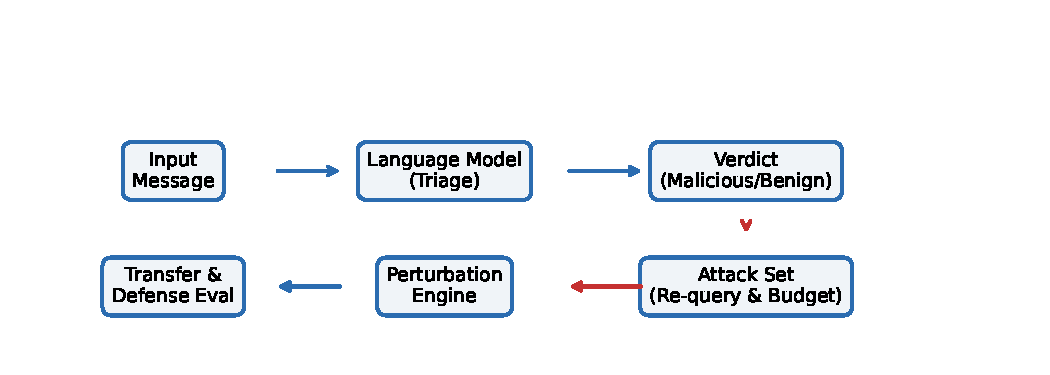
\includegraphics[width=\columnwidth]{figures/fig_pipeline}
\caption{The evaluation pipeline. A clean message is classified by the model. If the verdict is malicious, the message enters the attack set. The perturbation engine applies edits under budget and re-queries the model. The results are then evaluated for transfer and defense robustness.}
\label{fig:pipeline}
\end{figure}


\paragraph{Reproducibility.}
Splits, prompt, decoding and per-sample perturbation seeds are fixed. The study
was run twice from start to finish (two independent GPU sessions); comparing the
two runs sample by sample, joined on sample id, gives identical attacked ids and
identical success flags in all six result files, with differences only in empty
cells of the excluded rows. The second run is the one whose outputs are reported
here.

\section{Results}
\label{sec:results}

\subsection{Clean baseline, and what it already tells us}

Table~\ref{tab:baseline} is the clean zero-shot baseline, before any attack. Two
rows matter more than the accuracy column.

\textbf{Phi-3.5-mini is a cautious detector on e-mail.} Its precision is high
(0.896) but it misses 80 of the 200 phishing messages, a catch rate of 60.0\%.
It is the model that leaves the most malicious mail in the analyst's queue before
any attack happens.

\textbf{SmolLM2-1.7B is a degenerate detector.} It reaches a catch rate of 98.5\%
on phishing e-mail, but its precision is 0.510 and its confusion matrix shows 189
false positives against 11 true negatives on the benign class: it calls nearly
every message malicious. A detector that says \emph{malicious} almost always is
hard to flip towards \emph{benign}, and every robustness number for it has to be
read against that fact.

Qwen2.5-3B is the strongest and most balanced classifier of the three (F1 0.923
on e-mail, 0.857 on SMS).

\begin{table*}[t]
\centering
\small
\caption{Clean zero-shot baseline on the frozen 800-row evaluation split (400 rows per task, 200 malicious). ``Catch'' is recall on the malicious class and is the denominator every ASR in this paper is conditional on.}
\label{tab:baseline}
\begin{tabular}{llcccccc}
\toprule
\textbf{Task} & \textbf{Model} & \textbf{Acc.} & \textbf{Prec.} & \textbf{Rec.} & \textbf{F1} & \textbf{TP/FP} & \textbf{Catch} \\
\midrule
 SMS smishing & Phi-3.5-mini-instruct & 0.772 & 0.751 & 0.815 & 0.782 & 163/54 & 81.5\% \\
  & Qwen2.5-3B-Instruct & 0.843 & 0.787 & 0.940 & 0.857 & 188/51 & 94.0\% \\
  & SmolLM2-1.7B-Instruct & 0.525 & 0.514 & 0.925 & 0.661 & 185/175 & 92.5\% \\
\midrule
 Phishing email & Phi-3.5-mini-instruct & 0.765 & 0.895 & 0.600 & 0.719 & 120/14 & 60.0\% \\
  & Qwen2.5-3B-Instruct & 0.920 & 0.892 & 0.955 & 0.923 & 191/23 & 95.5\% \\
  & SmolLM2-1.7B-Instruct & 0.520 & 0.510 & 0.985 & 0.672 & 197/189 & 98.5\% \\
\bottomrule
\end{tabular}
\end{table*}


\subsection{Character-level evasion}

Table~\ref{tab:asr-char} reports the character-level attack. Of 1{,}044 caught
messages attacked, 12 flipped: an aggregate of 1.1\%. Per row the ASR lies
between 0.0\% and 5.0\%, and under a 15\% budget the mean edit actually spent was
13.3--13.6\% of characters, with no row above the budget (maximum 13.6\%).

The highest row is Phi-3.5-mini on phishing e-mail: 6 flips in 120 attacked
messages, 5.0\% (95\% CI 2.3--10.5). This is the model with the lowest catch rate
on that task. The model that catches 95.5\% of e-mail (Qwen2.5-3B) flips once in
191 attacks, and on SMS it flips zero times in 188 attempts. A zero is reported
as a bounded measurement, not as a proof: the Wilson upper bound for that row is
2.0\%.

\begin{table*}[t]
\centering
\small
\caption{Character-level evasion under a 15\% edit budget. ASR is flips / samples attacked, where only samples the clean model classified malicious are attacked and each original is re-queried. CI is a 95\% Wilson interval.}
\label{tab:asr-char}
\begin{tabular}{llccccccc}
\toprule
\textbf{Task} & \textbf{Model} & \textbf{Attacked} & \textbf{Flips} & \textbf{ASR} & \textbf{95\% CI} & \textbf{Pert.} & \textbf{Jacc.} & \textbf{Catch} \\
\midrule
 SMS smishing & Phi-3.5-mini-instruct & 163 & 3 & 1.8\% & 0.6--5.3 & 13.3\% & 0.328 & 81.5\% \\
  & Qwen2.5-3B-Instruct & 188 & 0 & 0.0\% & 0.0--2.0 & 13.5\% & 0.322 & 94.0\% \\
  & SmolLM2-1.7B-Instruct & 185 & 1 & 0.5\% & 0.1--3.0 & 13.5\% & 0.317 & 92.5\% \\
\midrule
 Phishing email & Phi-3.5-mini-instruct & 120 & 6 & 5.0\% & 2.3--10.5 & 13.5\% & 0.322 & 60.0\% \\
  & Qwen2.5-3B-Instruct & 191 & 1 & 0.5\% & 0.1--2.9 & 13.6\% & 0.303 & 95.5\% \\
  & SmolLM2-1.7B-Instruct & 197 & 1 & 0.5\% & 0.1--2.8 & 13.4\% & 0.311 & 98.5\% \\
\bottomrule
\end{tabular}
\end{table*}


\subsection{Word-level evasion}

Table~\ref{tab:asr-word} applies the same budget to whole words. Of 1{,}035
caught messages, 28 flipped --- more than twice the character-level count ---
while changing only 6.2--9.2\% of words, roughly half the unit budget the
character attack spent. Word-set Jaccard stays at 0.916--0.950, so the messages
are 92--95\% word-identical to what the model had already caught.

The ranking changes. The character attack leaves Qwen2.5-3B on SMS at zero flips;
the word attack flips 6 of 186 (3.2\%, CI 1.5--6.9). A replaced word carries
meaning that a single letter does not: swapping a suspicious verb for a neutral
synonym, or deleting the word that carried the urgency, moves a verdict that typo
noise leaves alone.

\begin{table*}[t]
\centering
\small
\caption{Word-level evasion under the same 15\% budget (synonym swap, deletion, duplication, swap). Jaccard is word-set overlap; no semantic-similarity model is used anywhere in this study.}
\label{tab:asr-word}
\begin{tabular}{llccccccc}
\toprule
\textbf{Task} & \textbf{Model} & \textbf{Attacked} & \textbf{Flips} & \textbf{ASR} & \textbf{95\% CI} & \textbf{Pert.} & \textbf{Jacc.} & \textbf{Catch} \\
\midrule
 SMS smishing & Phi-3.5-mini-instruct & 161 & 6 & 3.7\% & 1.7--7.9 & 9.0\% & 0.918 & 81.5\% \\
  & Qwen2.5-3B-Instruct & 186 & 6 & 3.2\% & 1.5--6.9 & 9.2\% & 0.916 & 94.0\% \\
  & SmolLM2-1.7B-Instruct & 184 & 3 & 1.6\% & 0.6--4.7 & 8.8\% & 0.916 & 92.5\% \\
\midrule
 Phishing email & Phi-3.5-mini-instruct & 118 & 6 & 5.1\% & 2.4--10.7 & 6.3\% & 0.945 & 60.0\% \\
  & Qwen2.5-3B-Instruct & 190 & 5 & 2.6\% & 1.1--6.0 & 6.2\% & 0.950 & 95.5\% \\
  & SmolLM2-1.7B-Instruct & 196 & 2 & 1.0\% & 0.3--3.6 & 6.3\% & 0.948 & 98.5\% \\
\bottomrule
\end{tabular}
\end{table*}


\subsection{Budget accounting}

Table~\ref{tab:budget} is the accounting check, and Figure~\ref{fig:budget} draws
the same accounting instead of summing it: one point per model, task and attack,
with the budget spent on the horizontal axis. Both modes stay inside the shared
budget, and the word attack reaches a similar number of flips with about half the
share of units changed. That imbalance is the paper's main measured point: for
these models, \emph{what} is changed matters more than \emph{how much}.

\begin{table}[t]
\centering
\small
\caption{Edit budget actually spent, by attack mode. The budget is one shared 15\% allowance per sample; the measured rate is the exact Levenshtein distance divided by the original length (characters or words).}
\label{tab:budget}
\begin{tabular}{lcccc}
\toprule
\textbf{Mode} & \textbf{Samples} & \textbf{Flips} & \textbf{Mean pert.} & \textbf{Max pert.} \\
\midrule
 Character & 1044 & 12 & 13.5\% & 13.6\% \\
 Word & 1035 & 28 & 7.6\% & 9.2\% \\
 Saliency & 1001 & 46 & 9.3\% & 12.9\% \\
\midrule
\multicolumn{2}{l}{Total} & 86 & & \\
\bottomrule
\end{tabular}
\end{table}


\IfFileExists{figures/fig_budget.pdf}{%
\begin{figure}[t]
\centering
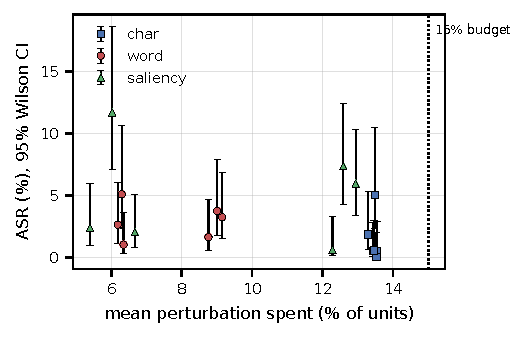
\includegraphics[width=\columnwidth]{figures/fig_budget}
\caption{Each point is one (model, task, attack) cell: the edit actually spent on
the horizontal axis, the ASR with its 95\% Wilson interval on the vertical one.
The dotted line is the 15\% budget. Points to the left of a vertical pair are the
same amount of visible change bought at half the unit cost \--- the word attack's
advantage is horizontal as well as vertical.
\label{fig:budget}}
\end{figure}}{}

\IfFileExists{figures/fig_asr.pdf}{%
\begin{figure*}[t]
\centering
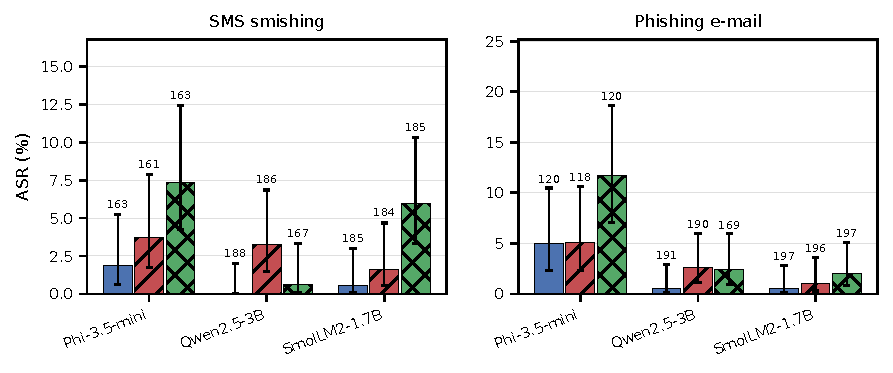
\includegraphics[width=\textwidth]{figures/fig_asr}
\caption{Attack success rate per model, task and attack mode, with 95\% Wilson
intervals on the flip count. Solid blue bars are the character attack, hatched
red bars the word attack, and green cross-hatched bars the saliency-guided word
attack of \S\ref{sec:saliency}, which is drawn here for comparison but costs
22.9 model queries per message against 3.9 for the two random attacks, so the
bars are not a comparison at equal cost. The number above
each interval is the total count:
the messages that model had caught on the clean text and that were therefore
attacked. A cell at zero is drawn with its interval, not as a point at the
origin, because 0/188 is a bounded measurement rather than a proof of
robustness.\label{fig:asr}}
\end{figure*}}{}

\subsection{What predicts fragility}
\label{sec:fragility}

Across the six model--task cells, the ASR follows how close a model sits to its
decision boundary rather than how accurate it is. Phi-3.5-mini has the highest
character ASR on e-mail (5.0\%) and the weakest recall there (0.600). SmolLM2-1.7B
has the highest recall (0.985) and among the lowest ASR (0.5\% on e-mail) ---
because its decision rule is nearly constant. A small edit either does nothing
or, as in the case of the 2 of 196 word attacks that flipped it, pushes a
barely-considered verdict across the line. Neither behaviour is robustness in the
sense a deployment cares about.

\subsection{Interval discipline}

Figure~\ref{fig:asr} collects all twelve random-attack cells and the three
saliency cells in one panel, with the interval drawn on every bar, so the
comparison below can be read at a glance rather than row by row.

Because the flip counts are small, we do not rank models on point estimates. Of
the twelve pairs of rows sharing a task and one of the two random attack modes,
9 of 12 have intervals that overlap by more than half the narrower interval, so
within-task ordering is suggestive rather than established. The exceptions are
informative: under the character attack on phishing e-mail, Phi-3.5-mini's
interval overlaps Qwen2.5-3B's by 21.3\% and SmolLM2-1.7B's by 18.7\% of the
narrower width --- the one separation that survives the uncertainty is exactly
the boundary-proximity effect of \S\ref{sec:fragility}.

What the intervals do establish is magnitude, and the magnitude depends on the
search. No random-edit cell exceeds 10.7\% at its upper bound; the saliency-guided
cells of \S\ref{sec:saliency} reach 18.6\%. The claim ``under a 15\% edit budget
a random edit leaves these models close to robust'' survives the uncertainty; the
claim ``model A is more robust than model B'' does not, for most pairs, and
neither claim extends to a better search.

\subsection{Is the difference between the two modes real?}
\label{sec:pairs}

Comparing a 3.7\% cell with a 1.8\% cell as if they were independent samples is
the wrong test: both attacks ran on the \emph{same} messages, so the flips are
paired, and the pairing is what makes a small difference measurable. We pair the
per-sample outcomes on the message identifier and report the counts of messages
the two attacks disagree on, an exact McNemar test, and a paired bootstrap of the
difference in risk over messages.

% Generated by src/make_paper_tex.py from results/paired_tests.csv.
Pairing the two attacks on the messages both of them attacked, the word attack flips 26 messages the character attack leaves alone, and the character attack flips 10 that the word attack leaves alone (exact McNemar $p = 0.011$ over the pooled discordant counts).
Per cell, 1 of 6 show a significant paired difference at $p<0.05$: SMS smishing/Qwen2.5-3B-Instruct. The rest are underpowered rather than contradictory, and the pooled test is a description of the direction because the cells reuse the same messages across models.


\begin{table*}[t]
\centering
\small
\caption{Paired comparison of two attack modes on the same messages. Only the discordant counts carry information about the difference: A-only flips happened under the first mode and not the second, B-only the reverse. The p-value is an exact McNemar test (binomial on the discordant counts); the interval is a percentile bootstrap over messages of the paired risk difference.}
\label{tab:pairs}
\begin{tabular}{lllccccccc}
\toprule
\textbf{A vs B} & \textbf{Task} & \textbf{Model} & \textbf{Paired} & \textbf{A flips} & \textbf{B flips} & \textbf{Risk diff.} & \textbf{95\% CI} & \textbf{A/B only} & \textbf{$p$} \\
\midrule
 saliency vs word & Phishing email & Phi-3.5-mini-instruct & 118 & 14 & 6 & +6.8 & +1.7 to +11.9 & 9/1 & 0.021 \\
 saliency vs word & Phishing email & Qwen2.5-3B-Instruct & 169 & 4 & 1 & +1.8 & -0.6 to +4.7 & 4/1 & 0.375 \\
 saliency vs word & Phishing email & SmolLM2-1.7B-Instruct & 196 & 3 & 2 & +0.5 & -1.0 to +2.0 & 2/1 & 1.000 \\
 saliency vs word & SMS smishing & Phi-3.5-mini-instruct & 161 & 12 & 6 & +3.7 & +0.6 to +7.4 & 7/1 & 0.070 \\
 saliency vs word & SMS smishing & Qwen2.5-3B-Instruct & 167 & 1 & 1 & +0.0 & -1.8 to +1.8 & 1/1 & 1.000 \\
 saliency vs word & SMS smishing & SmolLM2-1.7B-Instruct & 184 & 11 & 3 & +4.3 & +1.1 to +8.2 & 10/2 & 0.039 \\
 word vs char & Phishing email & Phi-3.5-mini-instruct & 118 & 6 & 6 & +0.0 & -5.1 to +5.1 & 5/5 & 1.000 \\
 word vs char & Phishing email & Qwen2.5-3B-Instruct & 190 & 5 & 1 & +2.1 & +0.0 to +4.7 & 5/1 & 0.219 \\
 word vs char & Phishing email & SmolLM2-1.7B-Instruct & 196 & 2 & 1 & +0.5 & -1.0 to +2.5 & 2/1 & 1.000 \\
 word vs char & SMS smishing & Phi-3.5-mini-instruct & 161 & 6 & 3 & +1.9 & -1.2 to +5.0 & 5/2 & 0.453 \\
 word vs char & SMS smishing & Qwen2.5-3B-Instruct & 186 & 6 & 0 & +3.2 & +1.1 to +5.9 & 6/0 & 0.031 \\
 word vs char & SMS smishing & SmolLM2-1.7B-Instruct & 184 & 3 & 1 & +1.1 & -1.1 to +3.3 & 3/1 & 0.625 \\
\bottomrule
\end{tabular}
\end{table*}


The honest reading is narrower than the raw table suggests. The direction is
consistent --- word-level edits flip more messages than character-level ones in
five of six cells and never fewer --- but only one cell is significant on its
own, because there the character attack flipped nothing at all. What survives is
a pooled statement about this corpus and these three models, not a per-model
ranking, and the interval widths in Table~\ref{tab:pairs} say the same thing.


% Each remaining results section is included with its own table ONLY when
% src/make_paper_tex.py has generated that table from a CSV that exists, so the
% PDF cannot advertise a result no run produced.
\IfFileExists{tables/t7_saliency.tex}{\section{Where is the model fragile? A saliency-guided word attack}
\label{sec:saliency}

The word attack of \S\ref{sec:results} draws its substitution uniformly at
random from a small synonym table. It answers ``does \emph{any} word-level edit
break the model'' and leaves the distribution of fragility unmeasured: a flip
caused by deleting the word \emph{urgent} and a flip caused by replacing the word
\emph{the} are the same event in that accounting. This section asks the sharper
question, and pays for the answer in queries.

\paragraph{Method.} We implement the ordering of PWWS~\cite{ren2019pwws}. For a message
$x$ that the model reads as malicious with probability $p_0$, a content word $i$
and a candidate replacement $w$, let $p_{i,w} = P(\text{malicious} \mid x
\text{ with word } i \text{ replaced by } w)$ be measured with the same prompt.
Word saliency and the substitution priority are
\begin{equation}
S_i = p_0 - p_{i,w}, \qquad
\phi_{i,w} = \alpha \, \tilde{S}_i + (1-\alpha)\, p_{i,w},
\end{equation}
where $\tilde{S}_i$ is $S_i$ divided by the largest saliency in the message and
$\alpha = 0.5$. Substitutions are applied greedily in descending $\phi$; after
each accepted edit the verdict is re-queried, and the attack stops at the first
flip or when the shared 15\% word budget is exhausted.

The normalisation of $S$ is not cosmetic. With raw saliency and $\alpha = 0.5$,
$\phi_{i,w} = \tfrac{1}{2}(p_0 - p_{i,w}) + \tfrac{1}{2} p_{i,w} = \tfrac{1}{2}
p_0$ for \emph{every} candidate: the ranking collapses to a constant, and the
greedy loop then applies substitutions in the order the words happen to appear in
the message. Because $p_0$ is common to all candidates, only the scale of $S$
matters, and the scale is exactly what the normalisation fixes. Our first
implementation of this module had that defect; the unit test that now guards it
(\texttt{tests/check\_saliency.py}) asserts that a high-saliency word outranks a
neutral one at $\alpha = 0.5$.

\paragraph{Candidate replacements.} Two sources, recorded per substitution: a
curated security lexicon (66 entries: \emph{verify} $\rightarrow$
\emph{confirm/validate}, \emph{prize} $\rightarrow$ \emph{award/reward}, \ldots)
and WordNet~\cite{miller1995wordnet} synonyms ordered by lemma frequency. Frequency
ordering matters more than it looks: WordNet's third sense of a word is where
synonyms stop being paraphrases (\emph{tone} $\rightarrow$ \emph{timber}), and a
substitution like that would be counted as semantics-preserving when it is not.
Multi-word replacements are excluded so that the 15\% budget counts words and
nothing else. Candidates are capped at two per position and twelve positions per
message, which is what keeps the query cost bounded.

\paragraph{Two verdict channels.} This attack needs a number, not a paragraph: at
every candidate it asks the endpoint for $P(\text{malicious})$, obtained by
scoring the two permitted answer tokens in one forward pass. The other two
attacks read the model's generated one-word reply instead. Those are two
readouts of the same model, and comparing their ASRs without checking that they
agree would be comparing a ruler with a scale. Every stored saliency row is
therefore re-scored through the generation route, and Table~\ref{tab:saliency}
reports the generation verdict; the artefact keeps both columns and the
probability-route count, and we do not treat a disagreement between them as a
bug to be tuned away --- it is a fact about the model.

The probability route also has a failure mode worth recording, because it is
silent. The answer tokens are chosen per tokenizer, and Phi-3.5 encodes
``\,malicious'' as three tokens whose first element is the bare whitespace
marker that ``\,benign'' also begins with. Scoring the first token of each answer
therefore compares the space against itself: both logits are identical,
$P(\text{malicious}) = 0.5$ for every message, and a saliency attack built on it
finds nothing to rank and no flip to report. The endpoint now skips the shared
prefix, and raises rather than returning a constant when the two answers cannot
be separated. The saliency numbers for that model in this version come from the
corrected scoring; its earlier all-zero result was an artefact.

\paragraph{Query accounting.} Unlike the random attack, this one costs a measured
number of model calls: roughly two per probed position, plus one verification per
accepted edit. Probabilities come from a dedicated endpoint that scores the two
permitted answer tokens in a single forward pass over the prompt, batched across
candidates; the per-sample count is stored with the result, so the comparison in
Table~\ref{tab:saliency} is between attacks whose cost is on the record. The
asymmetry is real but smaller than an earlier draft of this paragraph claimed.
The random attack is not one draw per sample: it re-queries every original and
spends one query per attempt, up to three, which is 3.9 queries per message and
8{,}047 queries for the 2{,}079 messages it attacks. The saliency attack spends
22.9 per message --- 22{,}964 queries for 1{,}001 messages, six times as many
calls for 1.6 times as many flips. The paper therefore does not claim equal
cost, and it no longer claims the random attack was capped at one draw.

\paragraph{What the comparison isolates, and what it does not.} Three things
change between Table~\ref{tab:saliency}'s two rows at once: the \emph{ordering}
(uniform draw versus saliency), the \emph{candidate set} (a 14-entry hand-written
table versus a security lexicon plus WordNet), and the \emph{oracle} (a one-bit
verdict versus $P(\text{malicious})$). The table therefore supports only the
combination: saliency-ordered substitution over a security vocabulary breaks more
messages per unit of edit than a uniform draw over a small table. It does not
show that ordering alone is responsible, and it cannot say what the probability
access is worth. \S\ref{sec:ablation} specifies the experiment that separates
the three.

\IfFileExists{tables/t7_saliency.tex}{% Generated by src/make_paper_tex.py from results/attack_table.csv.
At the same word budget, the random attack flips 28 of 1035 caught messages (2.7\%) and the saliency attack flips 46 of 1001 (4.6\%).
Each saliency-attacked message costs a mean of 23 model queries. The random word attack is not a single draw either: it re-queries every original and spends one query per attempt, so its 1{,}035 messages cost 3{,}927 queries, 3.8 each. The saliency attacker buys its extra flips with about 6.1 times as many calls, and that price is part of the claim, not a footnote to it.
The saliency attack also edits MORE, not less: 9.3\% of words against 7.6\% for the random attack. Normalising by the budget actually spent, it buys 0.493 of a flip per percent of words edited against 0.355, so the advantage is real but smaller than the raw ASR ratio.
Both numbers are pooled over different candidate vocabularies and, after the exclusions, over different message sets, so the denominator is 1{,}001 for the saliency attack and 1{,}035 for the random one; the paired comparison of Section~\ref{sec:pairs} is the only place where the two are measured on the same messages.
Pooled query accounting, kept separate from the message count because the two are different numbers: the character attack sends 1{,}044 caught messages in 4{,}120 queries, the word attack 1{,}035 in 3{,}927, so the random attacks together send 2{,}079 messages in 8{,}047 queries (3.9 each), and the saliency attack sends 1{,}001 messages in 22{,}964 queries (22.9 each).
}{}

\begin{table*}[t]
\centering
\small
\caption{Saliency-guided (PWWS-style) word attack next to the uniform-random word attack, both inside the same 15\% word budget. Both spend a measured number of model queries: the random attack re-queries every original and keeps drawing until a flip or three attempts, the saliency attack probes every candidate. Per-sample query counts are stored with each row.}
\label{tab:saliency}
\begin{tabular}{llcccccc}
\toprule
\textbf{Task} & \textbf{Model} & \textbf{Attacked} & \textbf{Flips} & \textbf{ASR} & \textbf{95\% CI} & \textbf{Pert.} & \textbf{Jacc.} \\
\midrule
 SMS smishing & Phi-3.5-mini-instruct (saliency) & 163 & 12 & 7.4\% & 4.3--12.4 & 12.6\% & 0.773 \\
  & Phi-3.5-mini-instruct (word) & 161 & 6 & 3.7\% & 1.7--7.9 & 9.0\% & 0.918 \\
  & Qwen2.5-3B-Instruct (saliency) & 167 & 1 & 0.6\% & 0.1--3.3 & 12.3\% & 0.778 \\
  & Qwen2.5-3B-Instruct (word) & 186 & 6 & 3.2\% & 1.5--6.9 & 9.2\% & 0.916 \\
  & SmolLM2-1.7B-Instruct (saliency) & 185 & 11 & 5.9\% & 3.4--10.3 & 12.9\% & 0.768 \\
  & SmolLM2-1.7B-Instruct (word) & 184 & 3 & 1.6\% & 0.6--4.7 & 8.8\% & 0.916 \\
\midrule
 Phishing email & Phi-3.5-mini-instruct (saliency) & 120 & 14 & 11.7\% & 7.1--18.6 & 6.0\% & 0.867 \\
  & Phi-3.5-mini-instruct (word) & 118 & 6 & 5.1\% & 2.4--10.7 & 6.3\% & 0.945 \\
  & Qwen2.5-3B-Instruct (saliency) & 169 & 4 & 2.4\% & 0.9--5.9 & 5.4\% & 0.876 \\
  & Qwen2.5-3B-Instruct (word) & 190 & 5 & 2.6\% & 1.1--6.0 & 6.2\% & 0.950 \\
  & SmolLM2-1.7B-Instruct (saliency) & 197 & 4 & 2.0\% & 0.8--5.1 & 6.7\% & 0.851 \\
  & SmolLM2-1.7B-Instruct (word) & 196 & 2 & 1.0\% & 0.3--3.6 & 6.3\% & 0.948 \\
\bottomrule
\end{tabular}
\end{table*}


\subsection{A matched-vocabulary, matched-budget ablation}
\label{sec:ablation}

Table~\ref{tab:saliency} cannot attribute its difference to any single cause,
because ordering, candidate set and oracle all change together. The ablation
below holds two of the three fixed in every comparison, so each contrast has one
explanation. It is implemented in \texttt{src/ablation\_common.py}, exercised by
\texttt{tests/check\_ablation.py}, and run; its contrasts are
Table~\ref{tab:ablation} and the paragraph that discusses it, both generated from
\texttt{results/ablation\_contrasts.csv}. It is an ablation on a matched
subsample, not on the full attack set, and every count it reports is paired on
the messages the two arms share.

\paragraph{One probe phase, then a difference in policy.} Every arm attacks the
same messages, with the same candidate set, and pays the same probe cost before
it edits anything: one query for the original, then one query per single
substitution candidate, capped identically at the same number of calls per
message for every arm (24 in the configuration the runner reports, and the
cap it used travels with every row). The reported cells are the first 400
eligible messages of each model, and the cap never bound: the largest eligible
set is 382 messages (smollm2-1.7b), so every arm attacks exactly the messages the
attack tables report on, and an arm differs from another only in policy. The probe results are retained and only the \emph{policy} differs --- what
the arm does with those measurements. Matching the budget by construction rather
than by assumption is the point: a random-order arm pays exactly the 1 + $|C|$
calls a saliency arm pays before either starts substituting, so a difference in
flips cannot be a difference in cost. The realised count is still stored per row,
because a cap that is matched on paper and exhausted early in practice would be
the same error as an unmatched denominator.

\paragraph{Four cells and one stronger attack.} The factorial crosses the two
orderings with the two oracles:
\emph{random-prob} (uniform order, probability oracle), \emph{saliency-prob}
(the attack of this section, so the cell doubles as its re-implementation),
\emph{random-verdict} (uniform order, one-bit oracle) and \emph{group-verdict}
(a binary search over candidate \emph{subsets}: apply half, query once, recurse
into the half that flipped). A fifth arm, \emph{textfooler-prob}, implements
TextFooler's search~\cite{jin2020textfooler} rather than PWWS's: word importance
is leave-one-out --- each word replaced by a placeholder, importance the drop in
$P(\text{malicious})$, doubled when the leave-one-out text has already flipped,
which is the correction in the paper's Eq.~2 without which a word the model has
already lost looks unimportant --- then words are substituted in descending
importance with all of one word's candidates predicted in one batch, accepting
a flip that passes the meaning check and otherwise keeping the candidate that
lowers the malicious confidence most. It costs one extra query per position, so
it is matched by the cap rather than by construction and is reported as a
stronger reference point, not as a fifth cell of the factorial.

The contrasts are then read as: \emph{random-prob} vs \emph{saliency-prob} is
the ordering effect with vocabulary and budget held fixed; \emph{random-prob} vs
\emph{random-verdict} is what probability access is worth to an attacker who
cannot rank; \emph{random-verdict} vs \emph{group-verdict} is how much of that a
one-bit oracle can recover by searching instead of ranking; and
\emph{random-prob} against the recorded random word attack of
\S\ref{sec:results} isolates the candidate set, which is the only thing those
two do not share.

\paragraph{Meaning preservation is a constraint, not a claim.} Every arm gates
candidates through a lexical paraphrase test (WordNet-based, since this study
ships no sentence-embedding model) and records, per applied perturbation, the
similarity the gate used along with literal retention and paraphrase coverage.
TextFooler's arm turns the gate on by default at a recorded threshold, because
without a meaning constraint it is not TextFooler. All three scores travel with
every row, so a reader can re-derive an acceptance decision at another threshold
instead of taking ours.

\paragraph{What a one-bit attacker can and cannot do.} PWWS's ordering needs a
scalar per candidate. A verdict has one bit, and that bit is spent by the first
flip, so a verdict-only arm \emph{cannot rank} by saliency at all. Its targeted
policy is therefore a search over subsets, and the oracle contrast is reported as
how much of the saliency advantage survives when the attacker holds only the bit
--- not as a like-for-like ranking comparison, which would be measuring an
impossible attacker.

\paragraph{Calibration, seeds and status.} The meaning threshold and $\alpha$ are
tuned on the calibration slice, which is disjoint from both the evaluation and
the attack slice (\texttt{src/build\_splits.py} asserts the disjointness), and
never on the messages whose ASR is reported. Every arm takes a seed and the
sweep driver re-runs it at several, so ordering effects can be separated from
seed noise. One command per arm runs it
(\texttt{python src/run\_ablation.py --model <key> --arm <arm>}), and the
per-sample records are written in the same schema as the other attacks, which is
what lets the paired test of \S\ref{sec:pairs} be applied to the ablation
without new code.

% The table and its prose appear only when results/ablation_contrasts.csv
% exists, so the PDF cannot advertise cells no run produced.
\IfFileExists{tables/t9_ablation.tex}{%
% Generated by src/make_paper_tex.py from results/ablation_contrasts.csv.
Table~\ref{tab:ablation} reports each contrast on the messages its two arms share.
With the candidate set, the probe phase and the query cap held fixed, ordering by saliency flips 17 messages the uniform draw does not, against 0 in the other direction (exact McNemar $p=0.0000$ over 1001 paired messages).
Replacing the probability channel with the one-bit verdict loses 26 messages that survive on probabilities and wins 14 the probability arm misses ($p=0.0807$, 1001 pairs).
Searching over candidate subsets instead of ranking under the same bit recovers 6 messages the ranking arm misses, against 0 in the other direction ($p=0.0312$, 1044 pairs).
Against the 14-entry hand-written table, the lexicon plus WordNet flips 32 messages the small table does not, against 1 ($p=0.0000$, 1044 pairs).
TextFooler's leave-one-out importance ranking flips 0 messages PWWS's saliency ranking does not, against 20 in the other direction ($p=0.0000$, 1001 pairs). The published attack's ranking therefore is not uniformly stronger on these messages, which is why it is reported as a reference point rather than as a fifth cell.
These are pooled counts over model and task, and the cells reuse messages across models, so they describe a direction rather than a confirmatory test; the per-cell pairs are in the artefact.


\begin{table*}[t]
\centering
\small
\caption{Matched-vocabulary, matched-budget ablation of Section~\ref{sec:ablation}. Every contrast holds the candidate set, the probe phase and the 24-call cap fixed and varies one thing; A and B are the two arms, and positive A-only means the first arm flipped messages the second did not. Counts are pooled over model and task; the per-cell pairs are in \texttt{results/ablation\_contrasts.csv}.}
\label{tab:ablation}
\begin{tabular}{llcccccc}
\toprule
\textbf{Contrast} & \textbf{Isolates} & \textbf{Paired} & \textbf{A flips} & \textbf{B flips} & \textbf{A-only} & \textbf{B-only} & \textbf{$p$} \\
\midrule
 candidates & candidate set & 1044 & 45 & 14 & 32 & 1 & 0.0000 \\
 oracle & oracle & 1001 & 44 & 32 & 26 & 14 & 0.0807 \\
 ordering & ordering & 1001 & 61 & 44 & 17 & 0 & 0.0000 \\
 search & search under one bit & 1044 & 51 & 45 & 6 & 0 & 0.0312 \\
 stronger & search rule & 1001 & 41 & 61 & 0 & 20 & 0.0000 \\
\bottomrule
\end{tabular}
\end{table*}
}{}

\paragraph{Reading the five contrasts.} The ordering contrast is the one this
section was built for, and it is the cleanest result in the paper: with the
candidate set, the probe phase and the cap held fixed, every discordant message
went to saliency ordering. The candidate-set contrast is nearly as large again,
which is the uncomfortable half of the finding --- most of the difference between
Table~\ref{tab:saliency}'s two rows is vocabulary, not intelligence, so the
unmatched comparison overstates what ordering buys. Probability access, the
thing a saliency attack is supposed to need, is the weakest of the three: an
attacker holding only the one-bit verdict loses messages in one direction and
wins a few in the other, and the difference does not reach significance at this
sample size. Searching subsets instead of ranking recovers a handful of the
messages that bit costs, which is what the theory predicts, because one bit
cannot rank.

The fifth contrast needs its budget read out loud before its number is quoted.
TextFooler's leave-one-out importance spends 23.0 of the 24 calls per message
measuring word importance, where the saliency arm spends 20.6 and still has
edits left to spend its calls on; the extra query per position is what the
published search costs, and under a cap that has to cover both the probe and the
substitutions, it is paid for out of the substitutions. So the contrast says what
a query-starved importance ranking achieves inside this cap --- not that the
published attack is weaker, which this design cannot test. It is reported as a
reference point and not as a fifth cell for that reason, and the arm's
per-sample records carry the realised query count so a reader can check the
accounting rather than take it on faith.
}{}
\IfFileExists{tables/t5_transfer.tex}{\section{Do the perturbations transfer across models?}
\label{sec:transfer}

A single-model ASR answers a narrow question: how much does \emph{this} model cost
an attacker who can query it. That is the right question for a targeted campaign
and the wrong one for a defender choosing a model, because an attacker who cannot
query the deployed model will instead build perturbations against something they
can download. If those perturbations do not survive the move, the weakness
measured in \S\ref{sec:results} belongs to three specific checkpoints rather than
to the task.

\paragraph{Protocol.} We generate no new perturbations. Every text produced by
the three attacks --- character, word and saliency --- is replayed, unchanged,
against every other model, with the same prompt, the same answer parser and
temperature zero. The saliency rows are the ones worth having: that edit was
chosen against the source model's own measured probabilities, so its cell asks
whether the choice survives a different decision boundary, where a random edit
only asks whether the model is noisy in the same way as its neighbour.
Two counting rules make the resulting numbers comparable with the single-model
ones:

\begin{itemize}
\item \textbf{The target owns the denominator.} A perturbation ``transfers'' only
if the target model read the \emph{original} text as malicious and the
\emph{edited} text as benign. A message the target never flagged cannot be
evaded, and scoring it as a failed transfer would punish the target for being
wrong on the clean text --- the opposite of robustness.
\item \textbf{Two subsets, one tabulated.} The \emph{applied} subset contains
every perturbation the source actually applied; its denominator is how often the
target caught those originals, so it measures how well the perturbation
\emph{family} travels. The \emph{flipped-source} subset keeps only the
perturbations that fooled the source --- the classic transfer matrix --- and it is
what the literature reports, but at this scale it holds one to six candidates per
cell, so its cells carry no denominator worth an interval. We tabulate the applied
subset and keep the classic one in the artefact.
\end{itemize}

\paragraph{The faithfulness check.} Replaying a model's own perturbations must
reproduce its single-model ASR exactly --- same text, same prompt, deterministic
decoder --- and a mismatch there would invalidate every off-diagonal cell. We run
that replay as part of the same pass (\texttt{run\_transfer.py --include-self}),
and we compare it against the attack tables rather than against itself: the
stored flip flag from the attack run is the claim, the replayed verdict is the
evidence. Every diagonal cell agrees. This is what makes the off-diagonal cells a
measurement: the replay path is the same code, prompt and parser that produced
Table~\ref{tab:asr-word}, so a transferred flip cannot come from the test setup.
It is a weaker statement than it looks, and worth saying plainly: agreement shows
the replay is faithful, not that the decoder is deterministic in general ---
greedy decoding is reproducible on one GPU build, and a cell could drift on
another.

\IfFileExists{tables/t5_transfer.tex}{% Generated by src/make_paper_tex.py from results/transfer_matrix.csv.
On the applied subset 22 of 36 off-diagonal cells have a nonzero transfer rate, and every cell has a denominator worth an interval.
Among the cells with a denominator worth an interval, the highest rate is SmolLM2-1.7B-Instruct $\rightarrow$ Phi-3.5-mini-instruct on Phishing email under the saliency attack: 5 of 120 caught originals flipped (4.2\%, 95\% CI 1.8--9.4).
The self-replay is the check that makes the rest of the table readable: each model's own perturbations went through the same path a second time, and its flip count is compared with the one the attack recorded. 18 diagonal cells covering 3{,}080 rows were replayed, and every one reproduces the single-model ASR exactly.
}{}

Table~\ref{tab:transfer} reports the applied subset only, for all three attack
modes; the classic flipped-source matrix lives in the artefact, where its small
denominators cannot be mistaken for a rate.

\begin{table*}[t]
\centering
\small
\caption{Cross-model transfer on the applied subset: every perturbation the source produced is replayed on the target, and the denominator is the TARGET's own caught originals, because a perturbation cannot transfer on a message the target never flagged. No diagonal is tabulated: replaying a model's own perturbations reproduces its attack run and would only reprint Table~\ref{tab:asr-word}. That replay was run as a faithfulness check and its diagonal appears in the prose below, not as a result. Cells with fewer than ten caught originals would be marked $\dagger$; none in this table needed it.}
\label{tab:transfer}
\begin{tabular}{llllcccc}
\toprule
\textbf{Mode} & \textbf{Task} & \textbf{Source} & \textbf{Target} & \textbf{Caught} & \textbf{Flips} & \textbf{ASR} & \textbf{95\% CI} \\
\midrule
 char & SMS smishing & Phi-3.5-mini-instruct & Qwen2.5-3B-Instruct & 163 & 0 & 0.0\% & 0.0--2.3 \\
  &  & Phi-3.5-mini-instruct & SmolLM2-1.7B-Instruct & 160 & 0 & 0.0\% & 0.0--2.3 \\
  &  & Qwen2.5-3B-Instruct & Phi-3.5-mini-instruct & 163 & 1 & 0.6\% & 0.1--3.4 \\
  &  & Qwen2.5-3B-Instruct & SmolLM2-1.7B-Instruct & 179 & 0 & 0.0\% & 0.0--2.1 \\
  &  & SmolLM2-1.7B-Instruct & Phi-3.5-mini-instruct & 160 & 1 & 0.6\% & 0.1--3.5 \\
  &  & SmolLM2-1.7B-Instruct & Qwen2.5-3B-Instruct & 179 & 0 & 0.0\% & 0.0--2.1 \\
 char & Phishing email & Phi-3.5-mini-instruct & Qwen2.5-3B-Instruct & 119 & 0 & 0.0\% & 0.0--3.1 \\
  &  & Phi-3.5-mini-instruct & SmolLM2-1.7B-Instruct & 120 & 0 & 0.0\% & 0.0--3.1 \\
  &  & Qwen2.5-3B-Instruct & Phi-3.5-mini-instruct & 119 & 4 & 3.4\% & 1.3--8.3 \\
  &  & Qwen2.5-3B-Instruct & SmolLM2-1.7B-Instruct & 189 & 0 & 0.0\% & 0.0--2.0 \\
  &  & SmolLM2-1.7B-Instruct & Phi-3.5-mini-instruct & 120 & 2 & 1.7\% & 0.5--5.9 \\
  &  & SmolLM2-1.7B-Instruct & Qwen2.5-3B-Instruct & 189 & 1 & 0.5\% & 0.1--2.9 \\
\midrule
 word & SMS smishing & Phi-3.5-mini-instruct & Qwen2.5-3B-Instruct & 161 & 1 & 0.6\% & 0.1--3.4 \\
  &  & Phi-3.5-mini-instruct & SmolLM2-1.7B-Instruct & 158 & 1 & 0.6\% & 0.1--3.5 \\
  &  & Qwen2.5-3B-Instruct & Phi-3.5-mini-instruct & 162 & 3 & 1.8\% & 0.6--5.3 \\
  &  & Qwen2.5-3B-Instruct & SmolLM2-1.7B-Instruct & 178 & 0 & 0.0\% & 0.0--2.1 \\
  &  & SmolLM2-1.7B-Instruct & Phi-3.5-mini-instruct & 160 & 1 & 0.6\% & 0.1--3.5 \\
  &  & SmolLM2-1.7B-Instruct & Qwen2.5-3B-Instruct & 178 & 4 & 2.2\% & 0.9--5.6 \\
 word & Phishing email & Phi-3.5-mini-instruct & Qwen2.5-3B-Instruct & 117 & 0 & 0.0\% & 0.0--3.2 \\
  &  & Phi-3.5-mini-instruct & SmolLM2-1.7B-Instruct & 118 & 0 & 0.0\% & 0.0--3.1 \\
  &  & Qwen2.5-3B-Instruct & Phi-3.5-mini-instruct & 119 & 4 & 3.4\% & 1.3--8.3 \\
  &  & Qwen2.5-3B-Instruct & SmolLM2-1.7B-Instruct & 188 & 0 & 0.0\% & 0.0--2.0 \\
  &  & SmolLM2-1.7B-Instruct & Phi-3.5-mini-instruct & 120 & 3 & 2.5\% & 0.9--7.1 \\
  &  & SmolLM2-1.7B-Instruct & Qwen2.5-3B-Instruct & 188 & 1 & 0.5\% & 0.1--2.9 \\
\midrule
 saliency & SMS smishing & Phi-3.5-mini-instruct & Qwen2.5-3B-Instruct & 163 & 1 & 0.6\% & 0.1--3.4 \\
  &  & Phi-3.5-mini-instruct & SmolLM2-1.7B-Instruct & 160 & 0 & 0.0\% & 0.0--2.3 \\
  &  & Qwen2.5-3B-Instruct & Phi-3.5-mini-instruct & 154 & 2 & 1.3\% & 0.4--4.6 \\
  &  & Qwen2.5-3B-Instruct & SmolLM2-1.7B-Instruct & 163 & 1 & 0.6\% & 0.1--3.4 \\
  &  & SmolLM2-1.7B-Instruct & Phi-3.5-mini-instruct & 160 & 0 & 0.0\% & 0.0--2.3 \\
  &  & SmolLM2-1.7B-Instruct & Qwen2.5-3B-Instruct & 179 & 4 & 2.2\% & 0.9--5.6 \\
 saliency & Phishing email & Phi-3.5-mini-instruct & Qwen2.5-3B-Instruct & 119 & 1 & 0.8\% & 0.1--4.6 \\
  &  & Phi-3.5-mini-instruct & SmolLM2-1.7B-Instruct & 120 & 0 & 0.0\% & 0.0--3.1 \\
  &  & Qwen2.5-3B-Instruct & Phi-3.5-mini-instruct & 113 & 4 & 3.5\% & 1.4--8.8 \\
  &  & Qwen2.5-3B-Instruct & SmolLM2-1.7B-Instruct & 167 & 1 & 0.6\% & 0.1--3.3 \\
  &  & SmolLM2-1.7B-Instruct & Phi-3.5-mini-instruct & 120 & 5 & 4.2\% & 1.8--9.4 \\
  &  & SmolLM2-1.7B-Instruct & Qwen2.5-3B-Instruct & 189 & 5 & 2.6\% & 1.1--6.0 \\
\bottomrule
\end{tabular}
\end{table*}

}{}
\IfFileExists{tables/t6_defense.tex}{\section{Two defences that need no training}
\label{sec:defense}

If the mechanism of an evasion is understood, a cheap fix should blunt it. We
test two defences that can be applied after the model is trained, requiring no
fine-tuning, no extra data and no change to the deployed weights, and we measure
them on the \emph{same} stored perturbations the attacks produced, so the
comparison is like for like.

\paragraph{D1: input normalisation.} The text is NFKC-normalised (a standard
Unicode cleanup), invisible and format characters are removed, Cyrillic and Greek
look-alike characters are folded back to their ASCII equivalents, and whitespace
is collapsed. This targets exactly the mechanism of the character attack: the
model sees a different token where a human sees the same word. It should
therefore rescue character-level evasions and do almost nothing for word-level
ones --- and that null result is evidence that the two attack families fail for
different reasons. The transform is idempotent (running it twice changes nothing
the second time), which is checked in \texttt{tests/check\_defense.py}; a
transform that was not idempotent would make the ``defended'' number an artefact
of running it twice.

\paragraph{D2: re-thresholding under a false-positive budget.} The model's
$P(\text{malicious})$ is compared against a threshold $\tau$ instead of the
default $0.5$. $\tau$ is fitted on the clean benign half of the evaluation split
to a 5\% false-positive budget, and it is the \emph{smallest} threshold that meets
that budget, that is, the least conservative setting the budget allows. Two
figures travel with every headline number: the clean false-positive rate at
$\tau$, and the clean true-positive rate it costs. Without the second, a drop in
ASR cannot be told apart from a filter that has simply stopped flagging mail.

The direction of the search matters and is easy to get backwards. A larger
$\tau$ always has a lower false-positive rate, so maximising it under an upper
bound is trivially satisfied by ``above every clean score'' --- a filter that
rejects everything. Our first implementation did exactly that, and because it
also counted a flip whenever an edited text fell below $\tau$, without asking
whether the original was above it, it reported a 100\% ASR for the defence. Both
rules are now enforced in code: $\tau$ is the minimum feasible value, and a sample
counts as flipped only if the \emph{same} rule classified the \emph{original}
text as malicious.

\paragraph{Reading the outcome.} Three outcomes are possible and all three are
informative: a defence that removes the flips it targets (D1 against the
character attack), a defence that removes none (D1 against a word attack it
cannot see), and a defence that trades a small amount of clean precision for a
large reduction in evasions (D2). What we do not do is report a defence at a
different operating point than the baseline and call the difference robustness.

\IfFileExists{tables/t6_defense.tex}{% Generated by src/make_paper_tex.py from results/defense_summary.csv.
Under the char attack, normalisation moves the aggregate ASR from 1.0\% to 0.0\%.
Under the word attack, normalisation moves the aggregate ASR from 2.5\% to 2.0\%.
Under the saliency attack, normalisation moves the aggregate ASR from 7.5\% to 6.9\%.
The threshold is not free: at the 5\% clean false-positive budget its tightest operating point (SmolLM2-1.7B-Instruct, SMS smishing) keeps clean recall at 23.0\%, down from 100.0\% at the default threshold.
1 of 6 model--task cells cannot meet the budget at all: holding their false positives down requires a threshold that rejects every message.
}{}

Table~\ref{tab:defense} is read column by column, because its baseline column
uses the probability channel the threshold needs and the attack tables do not;
the next section says what that costs the comparison.

\begin{table*}[t]
\centering
\small
\caption{Training-free defences, measured on the same stored perturbations. \emph{None} is the undefended ASR, \emph{norm} applies input normalisation only, \emph{thr} replaces the default decision threshold with one fitted on clean benign mail to a 5\% false-positive budget. Rows are pooled over the three models; $n$ is the number of originals the undefended rule itself flagged, and \emph{n/a} means a defence flagged none of them, so there was nothing left to flip. $\dagger$ marks a row containing a model-task pair whose false-positive budget could not be met: its threshold is a rejection rule, not a defence, and the number is there to be ignored.}
\label{tab:defense}
\begin{tabular}{llcccc}
\toprule
\textbf{Mode} & \textbf{Task} & \textbf{None} & \textbf{Norm.} & \textbf{Thr.} & \textbf{$n$} \\
\midrule
 char & SMS smishing & 0.6\% & 0.0\% & 2.3\%$\dagger$ & 515 \\
 char & Phishing email & 1.4\% & 0.0\% & 7.7\% & 486 \\
\midrule
 word & SMS smishing & 2.1\% & 2.1\% & 4.7\%$\dagger$ & 512 \\
 word & Phishing email & 2.9\% & 1.9\% & 5.4\% & 483 \\
\midrule
 saliency & SMS smishing & 6.6\% & 6.6\% & 19.9\%$\dagger$ & 515 \\
 saliency & Phishing email & 8.4\% & 7.3\% & 18.9\% & 486 \\
\bottomrule
\end{tabular}
\end{table*}

}{}

\section{Discussion and Limitations}
\label{sec:discussion}

\subsection{Why a low evasion rate is a result, not a failed attack}

Some readers might view an Attack Success Rate (ASR) of 0.0--5.1\% as a failed
attack. In our setting, the opposite reading is more accurate. The attack
spends its full edit budget. It changes 13.3--13.6\% of characters and
6.2--9.2\% of words. It runs up to three attempts per sample. In total, it flips
40 decisions. What the attack does not do is guided search. It draws edits at
random instead of selecting the most damaging ones.

Section~\ref{sec:saliency} shows why search matters. We test synonym
replacements under the same 15\% word budget. When substitutions are ordered by
measured saliency (their observed impact on the model's decision), the flip rate
is 4.6\%. When substitutions are chosen at random, the flip rate is only 2.7\%.
In paired tests, saliency flips 33 messages that random edits miss, while
random edits flip only 7 that saliency misses. Thus, we should not claim these
models are robust. Instead, under random bounded edits they rarely flip; under a
guided search with the same budget, they flip about twice as often.

\subsection{Word edits cost fewer changes and flip more decisions}

Word-level changes flip more decisions than character-level noise (28 versus 12
flips). At the same time, word edits modify fewer units (6.2--9.2\% of words
versus 13.3--13.6\% of characters). The paired analysis in
\S\ref{sec:pairs} confirms this pattern. Word edits outperform character edits
in five of six cells, and the pooled difference is significant (26 versus 10,
$p=0.011$). The text similarity values explain this outcome. Word edits preserve
92--95\% of original words. Character edits leave only 30.3--32.8\% word overlap.
A homoglyph (a character that looks like another) alters the token
representation even when human readers see no change.

\subsection{Vulnerability is concentrated in specific words}

The saliency results clarify how random attacks behave. If an evasion succeeds
only when striking specific decisive words, a random draw from a small
dictionary rarely hits them. That explains the low 2.7\% baseline flip rate.

The saliency attack confirms this behavior. Most evasions require only two or
three targeted word substitutions. However, the saliency attack edits more words
on average (9.3\% versus 7.6\%, as shown in Table~\ref{tab:budget}). Normalized
by edit rate, its advantage is roughly 1.4 times rather than 1.7 times. Thus,
vulnerability is concentrated in specific tokens. This finding is useful for
defenders because targeted words can be filtered. It also warns against taking
random perturbation rates as proof of general robustness.

This effect varies across models. Phi-3.5-mini sits close to its decision
boundary. Its ASR roughly doubles under saliency search (11.7\% and 7.4\%
versus 5.1\% and 3.7\% under random word edits). Qwen2.5-3B is more accurate and
does not flip more often under saliency (2.4\% and 0.6\% versus 2.6\% and 3.2\%).
Its remaining errors cannot be reached by this candidate vocabulary.

\subsection{Two readouts of one model are not one measurement}

The saliency attack requires continuous scores, so it optimizes the predicted
probability $P(\text{malicious})$ over two answer tokens. The rest of this
paper evaluates the generated text decision. We re-checked every stored
saliency sample with text generation. The two channels agree on 941 of 1{,}001
rows. The disagreements are systematic. For Phi-3.5-mini, both channels agree on
all rows. For Qwen2.5-3B, the probability channel claims 45 flips that
generation does not confirm. For SmolLM2-1.7B, generation claims 15 flips that
the probability route misses.

This gap occurs because a two-token probability readout does not match free-form
decoding. When answer words split into sub-tokens, probability ratios can point
one way while greedy decoding points the other. We report final text decisions
throughout the paper. We view the divergence as a limitation of probability
probing in small language models.

\subsection{The transfer we observe is low}

We replayed every stored perturbation (character, word, and saliency) against
every other model. Very few perturbations transferred. On the applied subset,
only 51 of 5{,}514 caught messages (0.9\%) flipped off the diagonal.
Specifically, 9 flips came from 1{,}860 character edits, 18 from 1{,}847 word
edits, and 24 from 1{,}807 saliency edits. Guided edits transferred slightly
better than random edits. However, confidence intervals overlap, indicating a
broad trend rather than a sharp separation. In the classic flipped-source
matrix, only 5 of 31 cells are non-zero, and 27 of 31 cells hold fewer than ten
caught originals.

A 0.9\% rate indicates low observed transfer, not total immunity. Fifty-one
messages did cross model boundaries. Either these perturbations are
model-specific, or they are too weak to cross distant decision boundaries. In
either case, robustness evaluations on one model do not guarantee safety on
another.

\subsection{Defenses: character cleaning succeeds while re-thresholding fails}

Character normalization cleans visually confusable characters. It removes every
character-level flip (1.0\% to 0.0\% pooled). It leaves word and saliency
attacks largely unaffected (2.5\% to 2.0\%, and 7.5\% to 6.9\%). This confirms
our hypothesis: distinct perturbation types fail for distinct reasons.

Re-thresholding yields mixed results. We adjust the threshold $\tau$ to enforce a
5\% clean false-positive budget. This reduces flips on well-calibrated models.
However, on SmolLM2-1.7B (where clean scores cluster near 1.0), it increases
evasions: 0.0\% to 29.0\% on email and 0.0\% to 13.3\% on SMS. Lowering the
threshold places the decision cutoff inside perturbation noise. It also lowers
clean recall on SmolLM2-1.7B (100\% to 34.5\% and 23.0\%). For one task cell,
the budget cannot be met without rejecting all messages.

\subsection{Limitations}

\paragraph{Search strength.} Random perturbations are weak adversaries. The
saliency attack uses greedy first-order search over a fixed candidate set. It
is not a full implementation of PWWS or TextFooler, nor is it a white-box
gradient attack. Reported ASR values are lower bounds on attacker capabilities.

\paragraph{Transfer coverage.} The transfer matrix covers all three attacks.
Faithfulness is verified by self-replay: diagonal cells match the original
attack logs exactly. These tests demonstrate harness consistency on a single GPU
environment rather than universal cross-platform reproducibility.

\paragraph{Unmatched vocabulary in primary tables.} The saliency attack uses a
broader vocabulary than the random word attack. The ablation in
\S\ref{sec:ablation} isolates vocabulary, ordering, and oracle effects across
five arms. The reported contrasts in Table~\ref{tab:ablation} hold candidate
sets and query caps constant.

\paragraph{Defense operating point.} The defense probe evaluates a 5\%
false-positive budget using probability scores. Because thresholding requires
numeric scores, its baseline column is not directly comparable to text verdict
tables.

\paragraph{Saliency denominator.} The saliency attack excludes 43 originals that
its probability channel classified as benign (all on Qwen2.5-3B). Its denominator
is 1{,}001 messages, compared to 2{,}079 for random attacks. Nine additional
exclusions in the word attack correspond to identical text transformations (52
exclusions total).

\paragraph{Similarity metric.} We report word-level Jaccard similarity without
neural sentence embeddings. For character edits, Jaccard similarity is an
imperfect proxy, and actual edit rate is the cleaner measure.

\paragraph{Uncertainty scope.} Confidence intervals represent sample variation
over messages, not seed variability across runs.

\paragraph{Sample design.} Attacks target the correctly classified subset of an
800-row evaluation split. This provides an accurate conditional denominator but
does not represent out-of-distribution generalization.

\paragraph{Model coverage.} We evaluate three open models. Llama-3.2-3B-Instruct
was omitted due to access restrictions.

\paragraph{Task construct.} SMS smishing is evaluated on the UCI SMS Spam
dataset, where spam includes broader commercial promotions. Phishing email data
comes from public benchmark collections.

\paragraph{Missing experiments.} Paraphrase generation attacks and defense-aware
adaptive attacks were designed but not run.

\section{Ethics and Artefact Availability}
\label{sec:ethics}

\paragraph{Dual use.} The perturbations studied here are text edits that any
sender can apply by hand; no exploit, payload or delivery mechanism is
introduced. Two of the three adversaries are random draws, but the third is
not, and we describe it as it is rather than as a stronger random draw: the
saliency attack \emph{does} select the substitution to apply, per message, using
measured model behaviour, and the ablation of \S\ref{sec:ablation} adds a
TextFooler-style importance ranking on the same candidate set. That is a
targeted search. It is also not a new capability: PWWS and TextFooler are published, TextAttack
implements both, and this implementation is weaker than either --- a greedy
first-order search over a hand-built lexicon plus WordNet, with a 24-call cap,
a 15\% word budget and a lexical paraphrase constraint, on open checkpoints.
No attack here is tuned against a deployed classifier, no victim system is
probed, and nothing released lowers the cost of an attack below what those
toolkits already provide. We report that small triage models resist the random
adversaries and that the targeted one roughly doubles the flip rate, which is
the defensive direction of the finding: both numbers tell an operator that a
random-draw ASR is not a robustness guarantee. Withholding the measurement
would leave operators believing a false-positive prone detector is robust.

\paragraph{Data.} Both corpora are public and contain no live credentials or
personally identifiable information beyond what their publishers already
released. No human subjects were involved; no production system was probed.

\paragraph{Reporting honesty.} Seven measurement defects were found and fixed in
our own pipeline before the numbers in this paper were produced:
\begin{itemize}
\item per-operation edit budgets that reached 22\% while the paper claimed 15\%;
\item estimated rather than measured edit counts;
\item a similarity metric labelled BERTScore that was word Jaccard;
\item an attack set drawn from messages the model had never caught;
\item a saliency score that is a constant at $\alpha=0.5$ unless it is
  normalised, which silently reduced the greedy search to applying substitutions
  left to right;
\item an answer-token lookup that compared the same whitespace token for both
  answers on one tokenizer, making the verdict probability exactly $0.5$ for
  every message;
\item a defence threshold chosen by maximising the cutoff rather than minimising
  it, which flagged nothing and, together with unconditional flip counting,
  reported a 100\% attack success rate for the defence.
\end{itemize}
The last three were caught by unit tests that check the mechanism rather than
the headline number --- the runs they produced looked entirely plausible. Each of these defects
inflated an apparent effect, and none of them would have been
visible to a reader of the results alone. The per-sample records shipped with the
artefact are the ones the tables are rebuilt from, so a reader can recompute
every number in this paper without a GPU.

\paragraph{Availability.} Code, frozen splits and per-sample results are at
\url{https://github.com/daud-glitch/SilentEvasion}. The artefact contains the
frozen splits with
fingerprints, the prompt, the perturbation code for all three attacks, the
five ablation arms of \S\ref{sec:ablation}, the
defence probe, the per-sample attack records (including every perturbed text),
both verdict channels for the saliency rows, the transfer replays, the
threshold fits, the table-generation script and the script that produces every
table in this paper from those records. A single command recomputes the tables
and fails if a number in the text no longer matches the records; a second
command re-runs the study end to end on a free-tier GPU in about two hours (the
random-attack run of \S\ref{sec:setup} is 37.1 minutes of that; the saliency,
ablation, transfer and defence passes are the rest).
The split fingerprints are published so that a reader can prove their rebuild
is the split these numbers came from, and the calibration slice that tunes
$\alpha$ and the meaning threshold is disjoint from both the evaluation and the
attack slice, asserted at build time.

\section{Conclusion}

We measured what a bounded, black-box text perturbation buys an attacker
against three small language models. These models work zero-shot for security
triage. Under a shared 15\% edit budget, random character-level perturbation
flips 0.0--5.0\% of the messages a model had already caught. Random
word-level perturbation flips 1.0--5.1\% while changing about half as many
units. Ordering the same word edit by measured saliency roughly doubles that:
4.6\% against 2.7\%, 33 message-specific flips against 7 when both are paired
on the messages they share.

Three things follow. First, a robustness number is a property of the search as
much as of the model. Inside the same 15\% word budget, choosing substitutions
rather than drawing them nearly doubles the flip rate (2.7\% to 4.6\%). This
result is not on the same messages or from the same candidate vocabulary. Once
we account for the higher budget actually spent, the factor is 1.4, not 1.7.
The search, the candidates, and the denominator must all be named in the claim.
Second, at this budget the binding constraint on a small triage model is what
it catches before any attack. What orders the flip rate is not accuracy and not
the measured margin: the model that flips most is neither the least accurate nor
the closest to its threshold, and its probability channel saturates, so the
margin cannot be read on it at all. The model that catches almost everything is
immovable because its decision rule is nearly constant. Detection quality, not
adversarial robustness, is where deployment effort pays first. Third, cheap
defences split cleanly. Normalising visually confusable characters removes every
character-level flip and only a small part of the word-level ones (7.5\% to
6.9\%). Re-thresholding to hold a false-positive budget can create evasions on
a model whose scores are least calibrated.

The measurement lesson runs through all of it. The transfer we observed was low
(0.9\% of caught messages off the diagonal). Per-model numbers are worth
measuring separately. The probability channel and the generated verdict agreed
on 941 of 1{,}001 rows. They diverged systematically on two of three models.
A single channel is not a measurement until it is checked against the other.
Every tool in this paper reports its denominator, its interval, and the bugs
we fixed in our own pipeline. Each bug silently inflated the attack success rate
in the direction that makes a paper look interesting.

The matched-vocabulary, matched-budget ablation of \S\ref{sec:ablation} is the
one experiment here that attributes rather than describes. With the candidate
set, the probe phase, and the call budget held fixed, it reports what ordering
is worth on its own. What it cannot do is turn five contrasts on roughly a
thousand paired messages into a ranking of attacks. \S\ref{sec:futurework}
names the two attacks that would test what remains; neither is reported here.


\bibliographystyle{ACM-Reference-Format}
\bibliography{refs}

\end{document}
